\documentclass[11pt, oneside]{article}   	% use "amsart" instead of "article" for AMSLaTeX format
\usepackage{geometry}                		% See geometry.pdf to learn the layout options. There are lots.
\geometry{letterpaper}                   		% ... or a4paper or a5paper or ... 
%\geometry{landscape}                		% Activate for for rotated page geometry
%\usepackage[parfill]{parskip}    		% Activate to begin paragraphs with an empty line rather than an indent
\usepackage{graphicx}				% Use pdf, png, jpg, or eps� with pdflatex; use eps in DVI mode
								% TeX will automatically convert eps --> pdf in pdflatex		
\usepackage{amssymb, amsmath,amsthm}
\usepackage{algorithm}
\usepackage{algorithmic}


\newtheorem{theorem}{Theorem}
\newtheorem{lemma}[theorem]{Lemma}
\newtheorem{proposition}[theorem]{Proposition}
\newtheorem{corollary}[theorem]{Corollary}
\newtheorem{claim}[theorem]{Claim}
\newtheorem{definition}[theorem]{Definition}

\title{Minimum Spanning Trees over Bregman Divergences}
\author{Bill March}
%\date{}							% Activate to display a given date or no date

\begin{document}
\maketitle
%\section{}
%\subsection{}

\section{Defining the Problem}

The goal is to come up with an efficient and practical hierarchical clustering algorithm for Bregman divergences.  In general, we would like to build on my fast EMST algorithm to do this.  

One easy approach is to define a graph on points, with edge weights related to pairwise Bregman divergences.  Given this, it becomes simple to develop an MST algorithm.

Possible definitions of the graph:
\begin{itemize}
\item The weight on edge $(u,v)$ is $\min \left\{ d(u,v), d(v,u) \right\}$.  Pros: simple, easy to compute?.  Cons: ignores the directionality of the divergence. Also, means we always have to compute both ways when doing a prune or distance check. Actually, this fits in naturally, since every point appears separately as a query and as a reference. 
\item Impose a total ordering on the inputs (i.e. their index in the data matrix). Then, the edge weight is always computed with the lower index as the first argument of the divergence. However, we might get a loop in one Boruvka step, since two components could be each others nearest neighbors, but want to add different edges. 
\item Edge $(u,v)$ has weight $d(u, v) + d(v, u) / 2$.  This is the standard way to turn the divergence into a metric, I believe. 
\end{itemize}


Dual-tree algorithms using Bregman ball trees should be simple. Cayton's second paper gives algorithms to determine containment and intersection of two balls.  We can define the dual-tree NN search problem to be a ball intersection query.  Given a query node with bounding ball $B(q, d_q)$ and reference node $B(r, d_r)$, let $\hat{d}$ be the maximum distance to a nearest neighbor candidate over query points.  Then, we can prune if $B(q, d_q + \hat{d})$ doesn't intersect $B(r, d_r)$ (or we could add the distance on the other side).  

Does this somehow invoke the triangle inequality? I believe it does.  We are saying that any point that is closer to a point in the query than $\hat{d}$ must lie in $B(q, d_q + \hat{d})$. But, without the triangle inequality, a point could be far from $q$ but close to a point in $B(q, d_q)$? 

I may be able to get around this with the analog to the Pythagorean theorem for Bregman divergences. 

\begin{theorem}
\textbf{Pythagorean Thm. for Bregman Divergences.}
Let $C$ be a convex set and let $x \in C$. Then, for any $z$, we have 
\begin{equation}
d_f(x,z) \geq d_f(x,y) + d_f(y,z)
\end{equation}
where $y = \arg \min_{y \in C} d_f(y,z)$ is the projection of $z$ onto $C$.
\end{theorem}

Let $B(\mu_r, R_r)$ and $B^\dagger(\mu_q, R_q)$ be two Bregman balls.  (To-do: show that $B^\dagger$ is convex).

Goal: show that the minimizer $\hat{r}$ in $B$ to $\mu_q$ and $\hat{q}$ in $B^\dagger$ to $\mu_r$ are the minimizers of the pairwise distances. 

Bound $d(q, r)$ such that $q \in B^\dagger(\mu_q, R_q)$ and $r \in B(\mu_r, R_r)$.  






Rather than adding to the radius inside the definition of the ball (which requires the triangle inequality), I can use this?



Another possibility is to generalize the proof about the shortest distance between a point and a Bregman ball to the shortest distance between two Bregman balls. 


\subsection*{Symmetrizations of the Bregman divergence}

Possible symmetrizations of the Bregman divergence $d_f(x, y)$ induced by a convex and strictly differentiable functions $f$ (note that $d_f(x, y) = f(x) - f(y) - \langle x - y, \nabla f(y) \rangle$):
\begin{itemize}
\item Maximum: $\max(d_f(x,y), d_f(y, x)),$
\item Minimum: $\min(d_f(x,y), d_f(y, x)),$
\item Sum/average: $d_f(x,y) + d_f(y,x)$
\item Jensen Bregman divergence: $\frac{1}{2} \left(d_f\left(x, \frac{x + y}{2} \right) + d_f\left(y, \frac{x + y}{2} \right) \right) = \frac{1}{2}\left(f(x) + f(y)\right) + f\left(\frac{x + y}{2} \right)$
\end{itemize}
None of these symmetrizations result in a metric (fortunately or unfortunately). So it would be interesting/hard if we could devise pruning rules/bounds for each. 


%%%%%%%%%%%%%%

\subsection{Notation}

Since Bregman divergences are generally asymmetric, we'll need some terminology to determine whether we're interested in $d(x, y)$ or $d(y, x)$ for a given $x$ and $y$. 

We'll start by following Cayton's notation and define the \emph{left} Nearest Neighbor problem as the task of finding
\begin{equation}
x_q = \arg \min_x d_f(x, q)
\end{equation}
We will apply this convention throughout.  Therefore, the \emph{left} anything will refer to putting the ``reference'' on the left and the ``query'' on the right.  

In the case of balls, we think of the points in the set as ``queries'' and the centroid as the ``reference''.
Therefore, we define the \emph{right} Bregman Ball with center $\mu$ and radius $R$ to be the set 
\begin{equation}
B_r(\mu, R) = \{x : d(x, \mu) \leq R \}
\end{equation}
and the \emph{left} Bregman Ball with center $\nu$ and radius $R^\prime$ to be the set
\begin{equation}
B_l(\nu, R^\prime) = \{ x : d(\nu, x) \leq R^\prime \}
\end{equation}

With this convention in mind, we can define the left and right NN problem, and also left and right pruning rules.  A left pruning rule considers divergences of the form $d(x, q)$ for a query point $q$. 

%%%%%%%%%%%%

\section{Primitives on Bregman Ball Trees}

Projecting a point onto the surface of a ball
	this corresponds to closest point

Determine if one ball is contained in another 

Determine if two balls intersect


Want: min distance between two balls
	achieve this through two projections
	Prove something like observation of extension of Euclidean solution to this
	
Claim: distance between balls is bounded by distance between centers minus radii
	need to lower bound distance between balls
	So, no need to prove that we achieve this
	
Assume $\min_{q, r} d(q,r) < d(\mu_q, \mu_r) - R_q - R_r$.  Clearly, the balls don't overlap.
	Try applying Pythagorean theorem of Bregman divergences on q and r, wherever they are.
	
	Use definitions of balls (and fact that they are distinct: $d(q,\mu_r) > R_r$, etc.)



\subsection{Dual-Tree Pruning Rule}

\begin{definition}
The left and right Bregman balls with respect to a strictly convex function $f$ and Bregman divergence $d_f$ of radius $R$ and center $\mu$ are given by 
\begin{eqnarray}
B_f(\mu, R) & = & \{ x : d_f(x,\mu) \leq R \} \\
B_f^\dagger(\mu, R) & = & \{ x : d_f(\mu, x) \leq R \}
\end{eqnarray}
\end{definition}



\begin{lemma}
(Cayton) The minimizer $x_p$ of 
\begin{equation}
\min_{x \in B(\mu, R)} d_f(x, p)
\end{equation}
has the following properties:
\begin{enumerate}
\item $\nabla f(x_p) = \theta \nabla f (\mu) + (1 - \theta) \nabla f( p)$ for some $\theta \in [0, 1]$
\item $d_f(x_p, p) = R$
\item $d_f(x_p, \mu)$ is monotonic in $\theta$.
\end{enumerate}
\label{primal_ball_lemma}
\end{lemma}


We would like to prove an analogous claim in the other direction.
\begin{lemma}
The minimizer $y_t$ of 
\begin{equation}
\min_{y \in B_f^\dagger(\mu, R)} d_f(t, y)
\end{equation}
has the following properties:
\begin{enumerate}
\item $y_t = \eta \mu + (1 - \eta) t$ for some $\eta \in [0, 1]$ \label{dual_ball_lemma_claim_1}
\item $d_{f^*} (\nabla f(y_t), \nabla f(\mu)) = R$
\item $d_{f^*} (\nabla f(y_t), \nabla f(\mu))$ is monotonic in $\eta$. 
\end{enumerate}
\label{dual_ball_lemma}
\end{lemma}
\begin{proof}
We start with claim \ref{dual_ball_lemma_claim_1}. Using the identity between $d_f$ and $d_{f^*}$, we have that 
\begin{equation}
\min_{y \in B_f^\dagger(\mu, R)} d_f(t, y) = \min_{y \in B_f^\dagger(\mu, R)} d_{f^*}(\nabla f(y), \nabla f(t))
\end{equation}
Furthermore, we have that finding a minimizing $y$ in $B_f^\dagger(\mu, R)$ is equivalent to finding a minimizing $\nabla f(y)$ in $B_{f^*}(\nabla f(\mu), R)$ since the function $\nabla f$ is one-to-one.

Through this transformation, we can apply lemma \ref{primal_ball_lemma} to the divergence $d_{f^*}$ to obtain the other two parts of the lemma.
\end{proof}


We compute the (unknown) solution $(q^*, r^*)$ to
\begin{equation}
\min_{q \in B_f(\mu_q, R_q)} \min_{r \in B_f^\dagger(\mu_r, R_r)} d_f(q, r)
\label{eqn_dual_tree_opt}
\end{equation}
Using lemmas \ref{primal_ball_lemma} and \ref{dual_ball_lemma}, we can compute the points:
\begin{eqnarray}
\hat{q} & = & \arg \min_{q \in B_f(\mu_q, R_q)} d_f(q, \mu_r) \\
\hat{r} & = & \arg \min_{r \in B_f^\dagger(\mu_r, R_r)} d_f(\mu_q, r)
\end{eqnarray}

Applying the previous lemmas, we have that $r^*$ must be the projection of $q^*$ onto the ball around $\mu_r$ and vice versa. Therefore,
\begin{eqnarray}
\nabla f(q^*) & = & \theta \nabla f (\mu_r) + (1 - \theta) \nabla f(r^*) \\
d_f(q^*, \mu_q) & = & R_q \\
r^* & = & \eta \mu_q + (1 - \eta) q^*	 	\\
d_f(\mu_r, r^*) & = & R_r.
\end{eqnarray}

\noindent
\textit{Notes from 12/27 ...}
\paragraph*{Remark.} It is important to note that the above conditions are {\em necessary} for optimality. I have not yet been able to show that any pair $(\bar{q},\bar{r})$ that satisfies the above conditions, $d_f(\bar{q}, \bar{r}) = \min_{(q, r)} d_f(q, r)$ (so we lack {\em sufficiency} for this set of conditions). So what this implies is that even if we try to solve the problem in Equation \eqref{eqn_dual_tree_opt} with alternately solving the convex problems for $q$ and $r$. 

The projection $\hat{r}$ of $\mu_q$ onto $B^\dagger_f(\mu_r, R_r)$ and the projection $\hat{q}$ of $\mu_r$ onto $B_f(\mu_q, R_q)$ is given by the following set of equations (where we solve for $\alpha$ and $\beta$:
\begin{eqnarray}
\nabla f(\hat{q}) & = & \alpha \nabla f(\mu_r) + (1 - \alpha ) f(\mu_q) \\
d_f(\hat{q}, \mu_q) & = & R_q \\
\hat{r} & = & \beta \mu_q + (1 - \beta) \mu_r \\
d_f(\mu_r, \hat{r}) & = & R_r
\end{eqnarray}

If the operator $\nabla f$ were linear, we could simply apply it to the equation for $r^*$, then substitute to obtain an expression for $q^*$ in terms of $\mu_r$ and $\mu_q$. Unfortunately, this isn't necessarily the case (it is for L2, which is why our intuition holds up in that case). 

The linearization of $\nabla f$ is a lower bound for the true gradient? 

We know that $d_f(q^*, \mu_q) = R_q$ and that $d_{f^*} (\nabla f(r^*), \nabla f(\mu_r)) = R_r$. We also know that $d_f(\hat{q}, \mu_q) = R$ and that $d_{f^*}(\nabla f(\hat{r}, \nabla f(\mu_r))) = R_r$. Can we argue that there is only one such point on the boundary of the ball? 


Proof ideas:
\begin{itemize}
\item Show that the full optimization problem (Eqn.~\ref{eqn_dual_tree_opt}) is convex in both its arguments.  Then, consider a small perturbation away from $\hat{q}$ and $\hat{r}$.  For a small enough perturbation, we can replace the divergence of the perturbation with its linear expansion. (Actually, I think with convexity I can just claim that the linear Taylor series is always a lower bound, which should be all I need). We then show that the divergence of the perturbation is always larger than the original perturbation, so $(\hat{q}, \hat{r})$ must be the global minimum. 
\item Try to write down a counter example where $(q^*, r^*)$ are different from $(\hat{q}, \hat{r})$. 
\item Show that $d_f(q^*, r^*) \leq d_f(\hat{q}, \hat{r})$, then argue uniqueness from convexity.  (Although, we don't need uniqueness, since, we're just looking to bound the distance anyway).
\item Revisit the Pythagorean theorem about projections.  Write it down in primal and dual and see if something good happens.         
\end{itemize}


\subsubsection*{Possible counter examples}
Possible counter-example: 
KL Divergence: 

Need something where the bounding sets come close together but not along the line joining the means.

	One example: two ovals tilted toward each other.  These are convex sets, and the points minimizing the L2 distance between them are not on the line between the means. However, they are not balls. 
		Is there a Bregman divergence under which these sets are balls? Can Mahalanobis distance do this? 
		It will have to lack the triangle inequality

%%%%%%%%%%%%%%%%%%%%%%%%%%%%%%%%%%%%%%%%%%%%%%%%%%%%%%%%
%%%%%%%%%%%%%%%%%%%%%%%%%%%%%%%%%%%%%%%%%%%%%%%%%%%%%%%%
%%%%%%%%%%%%%%%%%%%%%%%%%%%%%%%%%%%%%%%%%%%%%%%%%%%%%%%%

First, we define left and right Bregman balls.

\begin{definition}
The left and right Bregman balls of radius $R$ and center $\mu$ are given by 
\begin{eqnarray}
B(\mu, R) & = & \{ x : d(x,\mu) \leq R \} \\
B^\dagger(\mu, R) & = & \{ x : d(\mu, x) \leq R \}
\end{eqnarray}
\end{definition}

Consider the all left-nearest-neighbors task.  For all $q$, find the $r$ that minimizes $d(r,q)$.

Let $B(\mu_r, R_r)$ and $B^\dagger(\mu_q, R_q)$ be Bregman balls enclosing the set of references and queries. Let each query $q$ have a candidate nearest neighbor $n_q$, with $d(n_q, q) = c_q$.  Let $c^* = \min_{q} c_q$.  

Then, we can prune this pair of nodes if 
\begin{equation}
\min_q \min_r d(r,q) > c^*
\end{equation}
So, we seek a lower bound on the quantity on the left.  If this lower bound is greater than $c^*$, we can prune.

We begin by applying the Pythagorean inequality.  Let $x_q$ be the projection of $q$ onto $B(\mu_r, R_r)$.  Then, we have for any $r \in B(\mu_r, R_r)$ and $q \in B^\dagger(\mu_q, R_q)$:
\begin{equation}
d(r, q) \geq d(r, x_q) + d(x_q, q)
\end{equation}
We lower bound the first term with 0.  Therefore, we can lower bound the distance between the two balls by computing 
\begin{equation}
\min_{q \in B^\dagger(\mu_q, R_q)} d(x_q, q) \text{, such that } d(\mu_q, q) \leq R_q
\label{eqn_lower_bd}
\end{equation}


\begin{claim}
The minimizer $\hat{q}$ of Eqn.~\ref{eqn_lower_bd} satisfies
\begin{equation}
\hat{q}^\prime = \rho \mu_q^\prime + (1 - \rho) \mu_r^\prime
\end{equation}
\end{claim}
\begin{proof}
As in the paper, we take the Lagrange dual of Eqn.~\ref{eqn_lower_bd}, differentiate, and set equal to zero.  This gives 
\begin{equation}
\nabla f(x_q) - \nabla f(q) + \lambda \nabla f(\mu_q) - \lambda \nabla f(q) = 0
\end{equation}
Plugging in the fact that $x_q^\prime$ lies on the line between $q^\prime$ and $\mu_r^\prime$, and solving for $q'$, we get
\begin{equation}
q^\prime = \frac{\theta}{\lambda + \theta} \mu_r^\prime + \frac{\lambda}{\lambda + \theta} \mu_q^\prime
\end{equation}
A change of variables completes the proof. 
\end{proof}

I think in order to show that the minimum can be found in the same way as the point to ball distance, I need to show that the solution lies on the boundary of the query ball, and that the function is monotonic in it's parameter $\rho$. 



\begin{algorithm}
\caption{\textbf{CanPruneDual}($\theta_l, \theta_r, c^*, \mu_q, R_q, \mu_r, R_r)$}
\begin{algorithmic}[5]
\STATE $\theta = \frac{\theta_l + \theta_r}{2}$
\STATE $x_\theta = \nabla f^*(\theta \mu_q^\prime + (1 - \theta) \mu_r^\prime ) $
\STATE $\mathcal{L}(\theta) = $
\end{algorithmic}
\label{alg_can_prune_dual}
\end{algorithm}


Idea: want to show that $c^* > d(q, r)$ for any $q$ and $r$ in their balls.

Take Lagrange dual, take derivatives w.r.t. $q$ and $r$, set equal to zero and solve.  Show by this that the optima lie on the line between the centroids.

Problem: get a weird second derivative popping up with $q$, not sure if I'm doing this right. Or, alternatively, if I apply the duality relationship, then I get just $q$ and $r$, which seems weird too.

There's no real reason for me to expect $q$ to behave like $r$ here. 

Just go through the calculus carefully again, I think I can make this work. Be careful not to insert any unnecessary $f$. 

%%%%%%%%%%%%%%%%%%%%%%%%%%%%%%%%%%%%%%%%%%%%%%%%%%%

\begin{theorem}
Let $r \in B(\mu_r, R_r)$ and $q \in B^\dagger(\mu_q, R_q)$.  Let $q^*$ and $r^*$ be the points in these balls that minimize $d(q, r)$ over all such pairs. Then, both $q^{* \prime}$ and $r^{* \prime}$ lie on the line between $\mu_q^\prime$ and $\mu_r^\prime$. 
\end{theorem}
\begin{proof}
If we are given $q^*$, then from Claim 2 in \cite{cayton} we have that $r^{* \prime}$ lies on the line between $q^{* \prime}$ and $\mu_r$. We can repeat this argument in the reverse direction to obtain two equations.  Substituting one into the other and applying a change of variables finishes the proof.

The proof will require a left sided version of Claim 2, which may not work out with derivatives correctly. 
\end{proof}



%%%%%%%%%%%%%%%%%

\section{Directed MST}

What is the MST on a directed graph, anyway?

What about this arboricity idea?

Don't forget that it's a complete graph -- this should make it much simpler.



%%%%%%%%%%%%%%%%%%%%

\section{Random Ideas}

Cayton's original paper mentions that building the tree bottom up might yield tighter bounds than the more efficient bottom down build.  We might be able to use our hierarchical clustering to improve the tree in this way, if there were some reason to do so.  


\begin{table}
\begin{tabular}{lccc}
\hline \\
Divergence & $\mathcal{X}$  & $f(x), x \in \mathcal{X}$ & $d_f(x, y), (x, y) \in \mathcal{X} \times \mathcal{X}$ \\ 
\hline \\
Squared Euclidean distance & $\mathbb{R}^d$ & $\frac{1}{2} \| x \|_2^2$ & $\frac{1}{2} \| x - y \|_2^2$ \\
Itakura-Saito  & $\mathbb{R}_+^d$ & $- \sum_i \log x_i$ & $\sum_i \left(\frac{x_i}{y_i} - \log \frac{x_i}{y_i} - 1 \right)$ \\
Kulback-Liebler & $d$-simplex & $\sum_i x_i \log_2 x_i $ & $\sum_i x_i \log_2 \frac{x_i}{y_i}$ \\
Generalized I-divergence & $\mathbb{R}_+^d$ & $\sum_i x_i \log x_i$ & $\sum_i x_i \log \frac{x_i}{y_i} - \sum_i (x_i - y_i)$ \\
\hline
\end{tabular}
\caption{Bregman divergences with generating functions}
\label{tab:bdivs}
\end{table}


\noindent
\textit{Notes from 12/27 ...}
\section*{Random Notes}
Notation:
\begin{itemize}
\item $B_f(\mu_q, R_q) = \{ x \colon d_f(x, \mu_q) \leq R_q \} = \{ x \colon d_{f^*}(\mu_q', x') \leq R_q \} = B^\dagger_{f^*}(\mu_q', R_q),$
\item $B^\dagger_f(\mu_r, R_r) = \{ x \colon d_f(\mu_r, x) \leq R_r \} = \{ x \colon d_{f^*}(x', \mu_r') \leq R_r \} = B_{f^*}(\mu_r', R_r),$
\item $(q^*, r^*) = \arg \min\limits_{q \in B_f(\mu_q, R_q), r \in B^\dagger_f(\mu_r, R_r)} d_f(q, r),$
  \begin{itemize}
  \item We can show that $q^* = \arg \min\limits_{q \in B_f(\mu_q, R_q)} d_f(q, r^*),$
  \item We can show that $r^* = \arg \min\limits_{r \in B^\dagger_f(\mu_r, R_r)} d_f(q^*, r) = \nabla f^*  \left(\arg \min\limits_{r' \in B_{f^*}(\mu_r', R_r)}  d_{f^*} (r',{ q^* }') \right) ,$
  \end{itemize}
\item Let $(\widehat{q}, \widehat{r})$ be the respective projections of $\mu_q$ and $\mu_r$ on their corresponding other balls:
  \begin{itemize}
  \item $\widehat{q} = \arg \min\limits_{q \in B_f(\mu_q, R_q)} d_f(q, \mu_r),$
    \begin{itemize}
    \item $\widehat{q}' = \theta_1 \mu_q' + (1 - \theta_1) \mu_r',$
    \item $d_f(\widehat{q}, \mu_q) = R_q,$
    \end{itemize}
  \item There exists another point at the intersection of the line joining $\mu_q'$ and $\mu_r'$ and the edge of $B^\dagger_f(\mu_r, R_r)$ we can call $\bar{r}$ such that:
    \begin{itemize}
    \item $\bar{r}' = \nu_1 \mu_q' + (1 - \nu_1) \mu_r',$
    \item $d_f(\mu_r, \bar{r}) = R_r,$
    \end{itemize}
  \item $\widehat{r} = \arg \min\limits_{r \in B^\dagger_f(\mu_r, R_r)} d_f(\mu_q, r),$
    \begin{itemize}
    \item $\widehat{r} = \theta_2 \mu_r + (1 - \theta_2) \mu_q,$
    \item $d_f(\mu_r, \widehat{r}) = R_r,$
    \end{itemize}
  \item There exists another point at the intersection of the line joining $\mu_q$ and $\mu_r$ and the edge of $B_f(\mu_q, R_q)$ we can call $\bar{q}$ such that:
    \begin{itemize}
    \item $\bar{q} = \nu_2 \mu_r + (1 - \nu_2) \mu_q,$
    \item $d_f(\bar{q}, \mu_q) = R_q.$
    \end{itemize}
  \end{itemize}
\end{itemize}

\begin{figure}[htb]
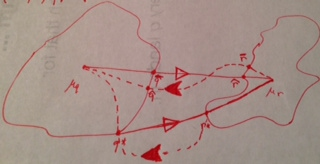
\includegraphics[width=\textwidth]{./images/notation}
\label{fig:notation}
\caption{{\bf Notation.} The solid line signifies a straight line in the primal space while the broken line denotes a straight line in the dual space.}
\end{figure}

\paragraph*{Random question.} Given a point $q$ and a convex set $B(\mu, R)$, let $x_q = \arg \min\limits_{x \in B(\mu, R)} d_f(x, q)$ be the projection of $q$ onto $B(\mu, R)$. We know that $x_q$ lies on the intersection of the line joining $\mu'$ and $q'$ and the edge of $B(\mu, R)$. If we have some other point $q_1$ such that $q_1'$ lies on the line joining $\mu'$ and $q'$, can we say that $\arg \min\limits_{x \in B(\mu, R)} d_f(x, q_1) == x_q$?
\begin{proof}
The answer is probably yes. This is because $x_{q_1} = \arg \min\limits_{x \in B(\mu, R)} d_f(x, q_1) $ lies at the intersection of the line joining $\mu'$ and $q_1'$ and the edge of $B(\mu, R)$ (that is, $d_f(x_{q_1}, \mu) = R$). This is the same line and the same Bregman ball for $x_q$. So $x_q == x_{q_1}$.
\end{proof}

\noindent
What this implies is that
\begin{itemize}
\item $ \widehat{q} = \arg \min\limits_{q \in B_f(\mu_q, R_q)} d_f(q, \mu_r) = \arg \min\limits_{q \in B_f(\mu_q, R_q)} d_f(q, \bar{r}) $
\item $\widehat{r} = \arg \min\limits_{r \in B^\dagger_f(\mu_r, R_r)} d_f(\mu_q, r) = \arg \min\limits_{r \in B^\dagger_f(\mu_r, R_r)} d_f(\bar{q}, r),$
\end{itemize}


Now we apply the Bregman Pythagorean theorem to all projections. 

\paragraph*{ISSUE}
The problem is that I was not able to get any useful (easy to compute) lower bound(s) on $d_f(q^*, r^*)$. The main issue is that $q^*$ and $r^*$ are projections of each other in the dual and primal space respectively, and hence there are no non-trivial inequalities using the Bregman Pythagorean theorem with the term $d_f(q^*, r^*)$ on the left hand side of the inequality\footnote{For clarity, let $C$ be a convex set and for any $x$, let $x_p = \arg \min_{z \in C} d_f(z, x)$ be the projection of $x$ onto $C$. Then the Pythagorean theorem tells us that $\forall y \in C, d_f(y, x) \geq d_f(y, x_p) + d_f(x_p, x)$.}.

\end{document}  